\newpage
\section{Auswertung}

\subsection{Quarzkügelchen}
    Für die weitere Auswertung ist es fundamental, die Auflösung der aufgenommenen Bilder zu kennen.
    Zu diesem Zweck wird die Größe eines Pixels in der CCD-Kamera-Software bestimmt.
    Die Größe der verwendeten Quarzkügelchen ist mit \qty{2,06}{\um} bekannt.
    Befindet sich nun ein Quarzkügelchen im Fokus des Mikroskops bzw. der Falle, wird es mit dem Zeichenwerkzeug markiert, siehe \autoref{fig:Pixelgroesse}.
    \begin{figure}[ht]
        \centering\captionsetup{format=plain}
        \includegraphics[width=0.5\textwidth]{bilder/Pixelgröße.JPG}
        \caption{Markierung eines eingefangenen Quarzkügelchens im Fokus des Mikroskops zur Bestimmung der Größe eines Pixels.}
        \label{fig:Pixelgroesse}
    \end{figure}
    \FloatBarrier
    Nach dem Zählen der Pixel entlang des Durchmessers des gelben Kreises ergibt sich die Pixelgröße zu
    \begin{equation}
        \mathrm{Pixelgröße} = \frac{\SI{2,06}{\um}}{122 \pm 4} \approx (16,9 \pm 0,6)\,\si{\nm} \;,
    \end{equation}
    wobei der Fehler durch das Festlegen des Randes der Quarzkugel zustande kommt.

\subsection{Kalibrierung der Spannung der Viersegment-Photodiode}
    Den Quarzkugeln wird NaCl-haltiges Wasser beigemischt.
    Die Kationen schirmen die elektrische Ladung der negativ geladenen Kugel ab, was ein Festkleben an den Wänden der Probenkammer wahrscheinlicher macht.
    Nun ist es möglich Messungen durchzuführen ohne, dass sich die Quarzkugeln bewegen.

    Zur Umrechnung des Spannungssignals der Viersegment-Photodiode in die tatsächliche Position in der Fokusebene des Mikroskops wurde die Optische Pinzette in x- und y-Richtung über eine fixierte Quarzkugel gescannt.
    Dabei wurde das auf der Photodiode gemessene Spannungssignal gegen die Position aufgetragen.
    Dies wurde für mehrere Laserleistungen durchgeführt, hier wird die Vorgehensweise exemplarisch nur für \qty{200}{mA} gezeigt.
    An den in \autoref{fig:PosCal_200mA} zu sehenden S-Kurven zwischen den blauen Linien wurden lineare Regressionen durchgeführt, um die Steigungen zu bestimmen.
    Diese geben die Konversationsfaktoren zwischen Photodiodenspannung und Position an.

    \begin{figure}[ht]
        \centering\captionsetup{format=plain}
        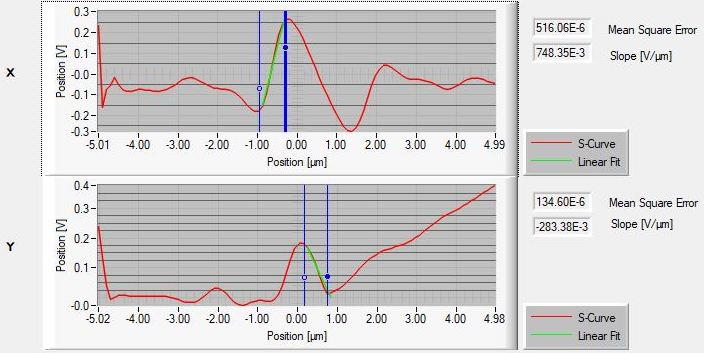
\includegraphics[width=0.6\textwidth]{bilder/PosCal_200mA.JPG}
        \caption{Ein Screenshot aus dem Thorlabs Programm im Menüpunkt \glqq \textit{position calibration} von einem Scan über eine fixierte Quarzkugel. Die Steigung der Flanken wird durch die grüne Gerade gefittet und gibt den Konversationsfaktor zwischen Photodiodenspannung und Position an.}
        \label{fig:PosCal_200mA}
    \end{figure}
    \FloatBarrier
    Trägt man die Konversationsfaktoren für verschiedene Laserleistungen auf, so ist kein deutlicher Trend zu erkennen.
    Es ist jedoch möglich die durchschnittlichen Konsversationsfaktoren für die x- und y-Richtung zu bestimmen:
    \begin{equation*}
        m_{\mathrm{x,konv}} \approx (0,71 \pm 0,05)\,\si{V \um^{-1}} \qquad m_{\mathrm{y,konv}} \approx (0,29 \pm 0.01)\,\si{V \um^{-1}}
    \end{equation*}
    \begin{figure}[ht]
        \centering\captionsetup{format=plain}
        \includegraphics[width=0.6\textwidth]{plots/Konversionsfaktoren.pdf} \vspace*{-0.5cm}
        \caption{Hier sind die Konversationsfaktoren für verschiedene Laserleistungen aufgetragen.}
        \label{fig:Konversionsfaktoren}
    \end{figure}
    \FloatBarrier
    Das in der Viersegment-Photodiode ankommende Summensignal, welches proportional zur einfallenden Gesamtintensität ist, wird zur Bestimmung der Position der Probenoberfläche genutzt.
    Dabei wird die axiale Position der Probenoberfläche relativ zum Fokus der Falle mit dem z-Piezo variiert.
    Der Ursprung der in \autoref{fig:Diodensumme} auf der x-Achse aufgetragenen z-Position wurde zufällig gewählt.
    Durch einen Vergleich mit der Theorie lässt sich die relative Position der Probenoberfläche grob bestimmen zu ca. \qty{33}{\um}.
    \begin{figure}[ht]
        \centering\captionsetup{format=plain}
        \includegraphics[width=0.6\textwidth]{plots/Diodensumme.pdf} \vspace*{-0.5cm}
        \caption{Zur Bestimmung der Position der Probenoberfläche wird das Diodensummensignal als Funktion der axialen Position der Probe und damit als Funktion der Position einer fixierten Quarzkugel gemessen.}
        \label{fig:Diodensumme}
    \end{figure}
    \FloatBarrier

\subsection{Fallensteifigkeit, Boltzmann-Konstante}
\subsubsection*{Ohne äußere Krafteinwirkung}
    Zur Bestimmung der Fallensteifigkeit werden Zeitserien der x- und y-Position einer nicht-fixierten eingefangenen Quarzkugel über eine Kalibrierungsdauer von $\Delta t_{\mathrm{cal}} = \qty{1}{s}$ aufgenommen.
    An die daraus bestimmte spektrale Leistungsdichte PSD kann eine Lorentzfunktion
    \begin{equation*}
        \mathrm{PSD}(f) = \frac{A}{f^2 + f_0^2}
    \end{equation*}
    gefittet werden, wie in \autoref{fig:PSD_keineKraft} zu sehen, die einen Wert für die sogenannte Roll-Off-Frequenz $f_0$ angibt.
    Aus dieser wiederum ergibt sich die Fallensteifigkeit
    \begin{equation*}
        k = 2 \pi \beta f_0 \quad \mathrm{mit} \quad \beta = 3 \pi \eta d \,,
    \end{equation*}
    wobei $\eta = \qty{8,9e-4}{\pascal \second}$ die Viskosität des fluiden Mediums und $d=\qty{2,06}{\um}$ der Durchmesser der Quarzkugeln ist.
    Dieses Verfahren ist exemplarisch in der \autoref{fig:PSD_keineKraft} und \ref{fig:k_keineKraft} für eine Laserstromstärke von \qty{150}{mA} verdeutlicht.
    Die Boltzmannkonstante wird über das Äquipartitionstheorem
    \begin{equation*}
        \frac{1}{2} k \langle x^2 \rangle = \frac{1}{2} k_B T \quad \Leftrightarrow \quad k_B = \frac{k}{T} \langle x^2 \rangle
    \end{equation*}
    bestimmt, wobei $\langle x^2 \rangle$ die statistische Varianz der Position des Kügelchens ist.
    Die x- und y-Positionen der Quarzkugel abhängig von der Zeit sind in \autoref{fig:pos_keineKraft} und die zugehörigen Leistungsdichten sind in \autoref{fig:PSD_keineKraft} dargestellt.
    Der grau hinterlegte Bereich markiert die Daten, an denen die Lorentzfunktion angepasst wurde.
    \begin{figure}[ht]
        \centering\captionsetup{format=plain}
        \includegraphics[width=0.8\textwidth]{plots/pos_keineKraft.pdf} \vspace*{-0.5cm}
        \caption{Die gemessenen Zeitserien der x- und y-Position sind hier dargestellt.}
        \label{fig:pos_keineKraft}
    \end{figure}
    \begin{figure}[ht]
        \centering\captionsetup{format=plain}
        \includegraphics[width=0.8\textwidth]{plots/PSD_keineKraft.pdf} \vspace*{-0.5cm}
        \caption{Die spektrale Leistungsdichte ist hier gegen die Frequenz aufgetragen. Eine Lorentzfunktion wird als Fit an die Daten angepasst.}
        \label{fig:PSD_keineKraft}
    \end{figure}
    % \FloatBarrier
    Es wurden allerdings auch Messungen bei den Laserstromstärken \qty{200}{mA}, \qty{250}{mA}, \qty{300}{mA} und \qty{350}{mA} durchgeführt, um eine lineare Abhängigkeit der Fallensteifigkeit von der Laserleistung zu untersuchen, die von Masaaki et al. in \cite{measurement_of_optical_trapping_force_gradient} gemessen wurde.
    An die Werte der Fallensteifigkeit in \autoref{fig:k_keineKraft} wurde jeweils eine lineare Regression
    \begin{equation}    
        \begin{aligned}
            k_x(P) &= \qty{6.45e-8}{\frac{\newton \; mW}{\metre}} \cdot P - \qty{2.05e-6}{\newton\per\metre} \\[4pt]
            k_y(P) &= \qty{5.08e-8}{\frac{\newton \; mW}{\metre}} \cdot P + \qty{6.96e-6}{\newton\per\metre}
        \end{aligned}
        \label{eqn:k_kalibrierung}
    \end{equation}
    angepasst.
    Der zweite Wert der Fallensteifigkeit wird dabei nicht beachtet, da die Varianz der Positionen sehr hoch ist und die berechneten Boltzmannkonstanten sehr stark vom Theoriewert von $k_b = \qty{1,38e-23}{\joule \kelvin^{-1}}$ abweichen, wie in \autoref{tab:keineKraftx} zu sehen ist.
    \begin{figure}[ht]
        \centering\captionsetup{format=plain}
        \includegraphics[width=0.6\textwidth]{plots/k_keineKraft.pdf} \vspace*{-0.5cm}
        \caption{Es sind die Werte der Fallensteifigkeiten ohne äußere Kraft abhängig von der Laserleistung aufgetragen. Eine Ausgleichsgerade wurde an die Daten angepasst.}
        \label{fig:k_keineKraft}
    \end{figure}
    \FloatBarrier
    \begin{table}[h]
        \centering
        \caption{Es sind die Werte der Fallensteifigkeit und der daraus berechneten Boltzmannkonstanten für verschiedene Laserleistungen in x-Richtung ohne äußere Krafteinwirkung gegeben.}
        \label{tab:keineKraftx}
        \begin{tabular}{c c c c}
        \toprule
        {$P$ [mW]} & {$\left\langle x^2 \right\rangle$ [$\mu \mathrm{m}^2$]} & {$k_\mathrm{x}$ [N/m]} & {$k_\mathrm{B,x}$ [J/K]}  \\
        \midrule
        \num{63.4}     &   \num{3.77e-4}   &   \num{5.53(26)e-6}	 &   \num{6.98(32)e-24}  \\
        \num{93.3}     &   \num{3.40e-1}   &   \num{1.09(27)e-6}	 &   \num{1.24(31)e-21}  \\
        \num{123.2}    &   \num{4.24e-3}   &   \num{4.13(15)e-6}	 &   \num{5.88(22)e-23}  \\
        \num{153.1}    &   \num{1.92e-4}   &   \num{6.08(12)e-6}	 &   \num{3.91(08)e-24}  \\
        \num{183.0}    &   \num{1.51e-4}   &   \num{1.27(03)e-5}	 &   \num{6.42(13)e-24}  \\
        \bottomrule
        \end{tabular}
    \end{table}

    \begin{table}[h]
        \centering
        \caption{Es sind die Werte der Fallensteifigkeit und der daraus berechneten Boltzmannkonstanten für verschiedene Laserleistungen in y-Richtung ohne äußere Krafteinwirkung gegeben.}
        \label{tab:keineKrafty}
        \begin{tabular}{c c c c}
        \toprule
        {$P$ [mW]} & {$\left\langle y^2 \right\rangle$ [$\mu \mathrm{m}^2$]} & {$k_\mathrm{y}$ [N/m]} & {$k_\mathrm{B,y}$ [J/K]}  \\
        \midrule
        \num{63.4}     &   \num{5.83e-5}   &  \num{1.20(03)e-5}    &  \num{2.35(07)e-24}  \\
        \num{93.3}     &   \num{6.10e+1}   &  \num{1.48(09)e-5}    &  \num{3.03(18)e-18}  \\
        \num{123.2}    &   \num{2.20e-3}   &  \num{6.33(31)e-6}    &  \num{4.66(23)e-23}  \\
        \num{153.1}    &   \num{5.47e-4}   &  \num{1.18(02)e-5}    &  \num{2.17(05)e-23}  \\
        \num{183.0}    &   \num{3.65e-4}   &  \num{2.11(05)e-5}    &  \num{2.58(06)e-23}  \\
        \bottomrule
        \end{tabular}
    \end{table}

\newpage
\subsubsection*{Mit äußerer Krafteinwirkung}
    Hier wurde eine Zeitserie aufgenommen, während die Probe sinusförmig in x-Richtung, d.h. $x = A \sin(2\pi f t)$ bewegt wurde, was die äußere Kraft darstellte.
    Die Bewegung geschah mit einer eingestellten Frequenz von \qty{1}{Hz} und einer Amplitude von \qty{5}{\um}.
    Bei der Bestimmung der Fallensteifigkeit wurde analog vorgegangen wie bei den Messwerten ohne Krafteinwirkung.
    Es wurden jedoch nicht die gleichen, sondern die anderen Laserstromstärken \qty{50}{mA}, \qty{70}{mA}, \qty{100}{mA}, \qty{150}{mA} und \qty{200}{mA} benutzt.

    \begin{table}[h]
        \centering
        \caption{Es sind die Werte der Fallensteifigkeit und der daraus berechneten Boltzmannkonstanten für verschiedene Laserleistungen in x-Richtung mit äußerer Krafteinwirkung gegeben.}
        \label{tab:mitKraftx}
        \begin{tabular}{c c c c}
        \toprule
        {$P$ [mW]} & {$\left\langle x^2 \right\rangle$ [$\mu \mathrm{m}^2$]} & {$k_\mathrm{x}$ [N/m]} & {$k_\mathrm{B,x}$ [J/K]}  \\
        \midrule
        \num{63.4}     &   \num{5.63e-2}   &   \num{2.00(09)e-6}	 &   \num{3.78(18)e-22}  \\
        \num{93.3}     &   \num{8.52e-3}   &   \num{2.53(08)e-6}	 &   \num{7.22(23)e-23}  \\
        \num{123.2}    &   \num{2.15e-3}   &   \num{1.87(14)e-6}	 &   \num{1.35(10)e-23}  \\
        \num{153.1}    &   \num{1.38e-2}   &   \num{2.52(11)e-6}	 &   \num{1.17(05)e-22}  \\
        \num{183.0}    &   \num{2.67e-4}   &   \num{1.11(03)e-5}	 &   \num{9.97(25)e-24}  \\
        \bottomrule
        \end{tabular}
    \end{table}

    \begin{table}[h]
        \centering
        \caption{Es sind die Werte der Fallensteifigkeit und der daraus berechneten Boltzmannkonstanten für verschiedene Laserleistungen in y-Richtung mit äußerer Krafteinwirkung gegeben.}
        \label{tab:mitKrafty}
        \begin{tabular}{c c c c}
        \toprule
        {$P$ [mW]} & {$\left\langle y^2 \right\rangle$ [$\mu \mathrm{m}^2$]} & {$k_\mathrm{y}$ [N/m]} & {$k_\mathrm{B,y}$ [J/K]}  \\
        \midrule
        \num{63.4}     &   \num{1.63e-1}   &  $(5,36 \pm \mathrm{inf}) \cdot 10^{-11}$   &  $(2,93 \pm \mathrm{inf}) \cdot 10^{-26}$  \\
        \num{93.3}     &   \num{7.46e-3}   &  \num{3.03(08)e-6}    &  \num{7.59(21)e-23}  \\
        \num{123.2}    &   \num{1.42e-3}   &  \num{3.77(19)e-6}    &  \num{1.79(09)e-23}  \\
        \num{153.1}    &   \num{3.89e-3}   &  \num{5.01(14)e-6}    &  \num{6.54(18)e-23}  \\
        \num{183.0}    &   \num{3.10e-4}   &  \num{1.13(02)e-6}    &  \num{1.18(02)e-23}  \\
        \bottomrule
        \end{tabular}
    \end{table}
    Anhand von \autoref{fig:PSD_mitKraft} ist zu erkennen, dass ein Lorentz-Fit nicht gut an den Messdaten anliegen kann und somit die Rolloffrequenz bzw. die Fallensteifigkeit für die Laserstromstärke \qty{50}{mA} einen sehr großen Fehler besitzt.
    Das Gleiche gilt auch für die stark abweichenden Werte der Fallensteifigkeiten in dem folgenden Abschnitt.
    Die Ausgleichsgeraden zur Darstellung der Laserleistungsabhängigkeit der Fallensteifigkeit in \autoref{fig:k_mitKraft} sehen wie folgt aus:
    \begin{align*}
        k_x(P) &= \qty{8.89e-8}{\frac{\newton \; mW}{\metre}} \cdot P + \qty{2.72e-7}{\newton\per\metre} \\[4pt]
        k_y(P) &= \qty{1.02e-7}{\frac{\newton \; mW}{\metre}} \cdot P + \qty{5.30e-7}{\newton\per\metre}
    \end{align*}
    Aus dem oben genannten Grund werden die stark abweichenden Werte nicht bei der linearen Regression betrachtet.
    \begin{figure}[ht]
        \centering\captionsetup{format=plain}
        \includegraphics[width=0.8\textwidth]{plots/PSD_mitKraft.pdf} \vspace*{-0.5cm}
        \caption{Die spektrale Leistungsdichte ist hier gegen die Frequenz aufgetragen. Eine Lorentzfunktion wird als Fit an die Daten angepasst.}
        \label{fig:PSD_mitKraft}
    \end{figure}
    \FloatBarrier
    \begin{figure}[ht]
        \centering\captionsetup{format=plain}
        \includegraphics[width=0.6\textwidth]{plots/k_mitKraft.pdf} \vspace*{-0.5cm}
        \caption{Es sind die Werte der Fallensteifigkeiten mit äußerer Kraft abhängig von der Laserleistung aufgetragen.}
        \label{fig:k_mitKraft}
    \end{figure}
    \FloatBarrier
    In \autoref{sec:discussion} wird darauf eingegangen, wieso die Stokes'sche Fallenkraft unter den gegebenen Umständen nicht bestimmt werden konnte.

\newpage
\subsubsection*{Mit äußerer Krafteinwirkung und Vortexretarder}
    Diese Messung ist fast identisch zu der Vorherigen, außer der Tatsache, dass ein Vortexretarder in den Strahlengang des Lasers der Falle eingesetzt wird.
    Das erzeugt einen optischen Vortex, d.h. das Laserlicht besitzt einen orbitalen Drehimpuls, der viel größer als der Spindrehimpuls $\pm\hbar$ pro Photon sein kann, welcher durch die zirkulare Polarisation des Lichtes gegeben ist.
    Die Übertragung des Photonenspins auf das eingefangene Teilchen verursacht eine Eigenrotation des Vesikels.
    Der orbitale Drehimpuls hingegen erzeugt eine Bewegung des Teilchens auf einer Kreisbahn um das Strahlzentrum herum, wie in \cite{optische_wirbel} beschrieben.
    Die Ermittlung der Fallenkraft ist aufgrund der gleichen Umstände wie im vorherigen Abschnitt nicht möglich.
    \begin{table}[h]
        \centering
        \caption{Es sind die Werte der Fallensteifigkeit und der daraus berechneten Boltzmannkonstanten für verschiedene Laserleistungen in x-Richtung mit äußerer Krafteinwirkung und eingesetzem Vortexretarder gegeben.}
        \label{tab:mitKraft_vortexx}
        \begin{tabular}{c c c c}
        \toprule
        {$P$ [mW]} & {$\left\langle x^2 \right\rangle$ [$\mu \mathrm{m}^2$]} & {$k_\mathrm{x}$ [N/m]} & {$k_\mathrm{B,x}$ [J/K]}  \\
        \midrule
        \num{4.8}     &   \num{3.77e-4}   &   \num{1.21(11)e-6}	    &   \num{2.28(22)e-22}  \\
        \num{15.6}    &   \num{3.40e-1}   &   $(8,08 \pm \mathrm{inf}) \cdot 10^{-11}$    &   $(2,31 \pm \mathrm{inf}) \cdot 10^{-27}$  \\
        \num{33.5}    &   \num{4.24e-3}   &   \num{1.34(15)e-6}	    &   \num{9.62(72)e-24}  \\
        \num{63.4}    &   \num{1.92e-4}   &   \num{3.38(10)e-6}	    &   \num{1.57(05)e-22}  \\
        \num{93.3}    &   \num{1.51e-4}   &   \num{5.98(13)e-6}	    &   \num{5.35(12)e-24}  \\
        \bottomrule
        \end{tabular}
    \end{table}

    \begin{table}[h]
        \centering
        \caption{Es sind die Werte der Fallensteifigkeit und der daraus berechneten Boltzmannkonstanten für verschiedene Laserleistungen in y-Richtung mit äußerer Krafteinwirkung und eingesetzem Vortexretarder gegeben.}
        \label{tab:mitKraft_vortexy}
        \begin{tabular}{c c c c}
        \toprule
        {$P$ [mW]} & {$\left\langle y^2 \right\rangle$ [$\mu \mathrm{m}^2$]} & {$k_\mathrm{y}$ [N/m]} & {$k_\mathrm{B,y}$ [J/K]}  \\
        \midrule
        \num{4.8}     &   \num{5.83e-5}   &  \num{1.81(08)e-6}     &  \num{9.90(43)e-22}  \\
        \num{15.6}    &   \num{6.10e+1}   &  $(1,36 \pm \mathrm{inf}) \cdot 10^{-10}$    &  $(3,39 \pm \mathrm{inf}) \cdot 10^{-27}$  \\
        \num{33.5}    &   \num{2.20e-3}   &  $(1,05 \pm \mathrm{inf}) \cdot 10^{-11}$    &  $(5,00 \pm \mathrm{inf}) \cdot 10^{-29}$  \\
        \num{63.4}    &   \num{5.47e-4}   &  \num{5.31(14)e-6}     &  \num{6.94(18)e-23}  \\
        \num{93.3}    &   \num{3.65e-4}   &  \num{1.01(02)e-5}     &  \num{1.05(02)e-23}  \\
        \bottomrule
        \end{tabular}
    \end{table}
    \begin{figure}[ht]
        \centering\captionsetup{format=plain}
        \includegraphics[width=0.6\textwidth]{plots/k_mitKraft_vortex.pdf} \vspace*{-0.5cm}
        \caption{Hier sind die Werte der Fallensteifigkeiten mit äußerer Kraft und eingesetztem Vortexretarder abhängig von der Laserleistung aufgetragen. Eine Ausgleichsgerade wurde an die Daten angepasst.}
        \label{fig:k_mitKraft_vortex}
    \end{figure}
    \FloatBarrier
    Die Ausgleichsgeraden in \autoref{fig:k_mitKraft_vortex} sehen wie folgt aus:
    \begin{align*}
        k_x(P) &= \qty{5.55e-8}{\frac{\newton \; mW}{\metre}} \cdot P - \qty{2.69e-7}{\newton\per\metre} \\[4pt]
        k_y(P) &= \qty{8.89e-8}{\frac{\newton \; mW}{\metre}} \cdot P - \qty{9.56e-7}{\newton\per\metre}
    \end{align*}
    Dabei werden die stark abweichenden Werte, also der Zweite in x-Richtung und der Zweite und Dritte in y-Richtung, nicht miteinbezogen.

\subsection{Vesikel in Zwiebelzellen}
    Es wurde der Tranport von Vesikeln in Zwiebelzellen beobachtet.
    Einige solcher Vesikel sind in \autoref{fig:Vesikel1} zu sehen.
    \begin{figure}[ht]
        \centering\captionsetup{format=plain}
        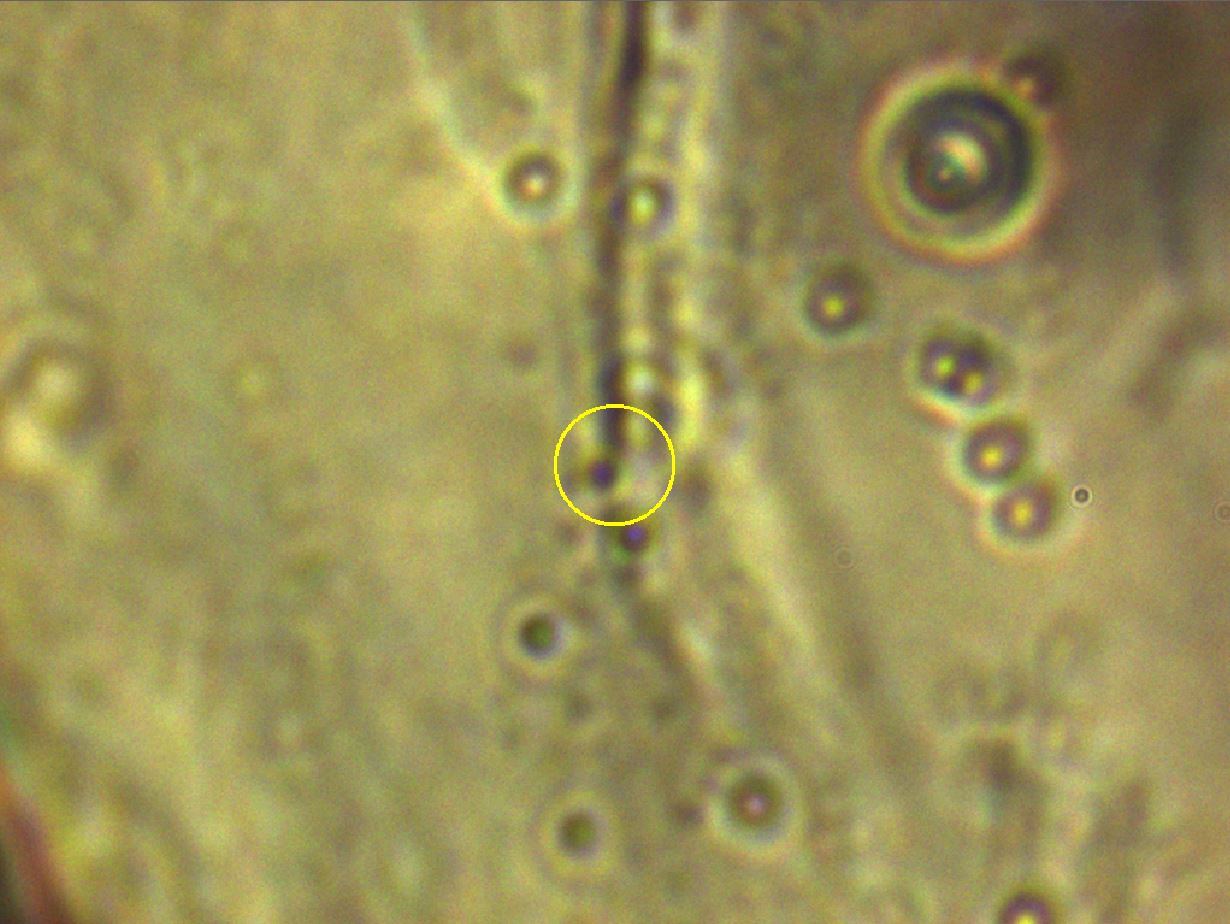
\includegraphics[width=0.5\textwidth]{bilder/Vesikel1.JPG}
        \caption{Mehrere Vesikel innerhalb einer Zwiebelzelle.}
        \label{fig:Vesikel1}
    \end{figure}
    \FloatBarrier
    Die Größe eines Vesikels wird mithilfe der schon bestimmten Pixelgröße in der Fokusebene festgestellt.
    Dafür wird ein Vesikelpfad gefunden, dessen Vesikel sich in der Fokusebene bewegen.
    Das wird erkannt, indem ein Vesikel dieses Pfades eingefangen wird, welches daraufhin nicht größer oder kleiner wird, also sich schon im Fokuspunkt der Falle befindet.
    In \autoref{fig:Vesikel_Groesse} ist das Vesikel als blau umrandeter Kreis zu erkennen.
    Es hat einen Durchmesser von \num{112(4)} Pixeln.
    Umgerechnet sind das ca. \qty{1.9(1)}{\um}.
    \begin{figure}[ht]
        \centering\captionsetup{format=plain}
        \includegraphics[width=0.5\textwidth]{bilder/Vesikel_Größe.png}
        \caption{Blau umrandetes Vesikel, wessen Größe bestimmt wurde.}
        \label{fig:Vesikel_Groesse}
    \end{figure}
    \FloatBarrier
    Eine Auslenkung der Vesikel durch die optische Falle ist möglich.
    Die maximale Fallensteifigkeit, die mit den gegebenen Laserleistungen erreicht werden kann, reicht jedoch nicht aus um sie komplett von der Aktin-Faser zu trennen.
    Nach dem Freilassen der Vesikel kehren diese zu ihrer ursprünglichen Position zurück und setzen ihre Bewegung nach ca. \qty{1}{s} wieder in gleicher Richtung fort.
    Eine weitere Beobachtung besteht darin, dass wenn ein Vesikel weit von seiner Aktin-Faser entfernt wurde, weitere Vesikel kurz an der Stelle der Auslenkung der Faser verlangsamt werden.

    Um die Geschwindigkeit der Vesikel zu bestimmen, wurde der Laser auf eine Aktin-Faser gerichtet.
    Dabei war die Laserleistung so stark reduziert, dass die Vesikel in ihrer Bewegung durch die Falle nicht eingeschränkt wurden.
    Das Diodensummensignal wurde abhängig von der Zeit aufgenommen, sodass aus der Dauer der Reduktion des Laserlichtes durch das sich vorbei bewegende Vesikel seine Geschwindigkeit $v$ berechnet werden kann.
    In \autoref{fig:Vesikel_Geschwindigkeit} ist solch eine Messung dargestellt.
    Im grau hinterlegten Intervall von $\Delta t = \qty{0.15(1)}{s}$ bewegt sich ein Vesikel durch den fokussierten Laserstrahl.
    Unter der Annahme, dass sich das Vesikel während der Reduktion des Laserlichtes um ein Zweifaches seines Durchmessers bewegt, ergibt sich eine Geschwindigkeit von $v = \qty{25.2(2.1)}{\um \per \second}$.
    \begin{figure}[ht]
        \centering\captionsetup{format=plain}
        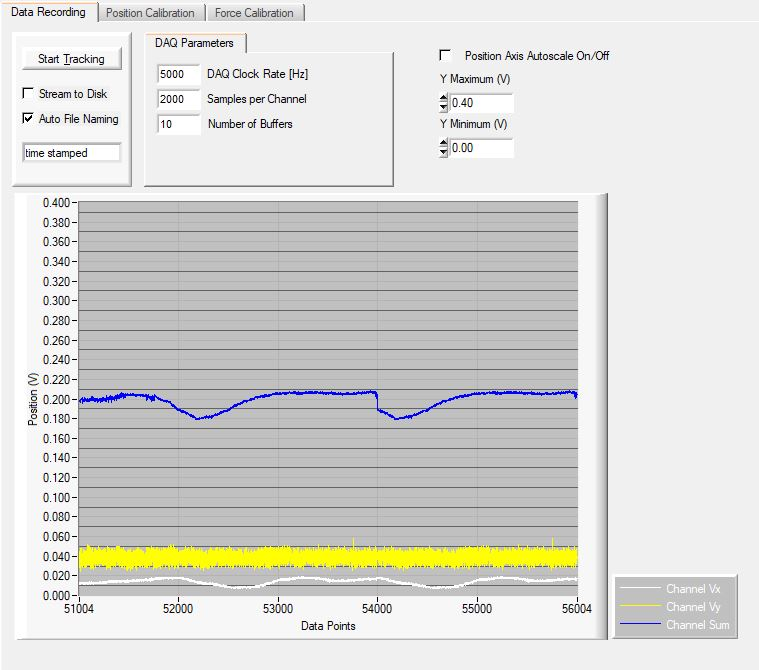
\includegraphics[width=0.6\textwidth]{plots/Vesikel_Geschwindigkeit.pdf} \vspace*{-0.5cm}
        \caption{Hier ist das Diodensummensignal gegen die Zeit aufgetragen, während zwei Vesikel hintereinander die Falle passieren.}
        \label{fig:Vesikel_Geschwindigkeit}
    \end{figure}
    \FloatBarrier

    Zur Bestimmung der Stärke der Aktin-Myosin-Motoren wurde die Falle auf einen Vesikelpfad fokussiert und die Laserleistung so weit hochgedreht, dass mindestens ein bewegtes Vesikel eingefangen wurde.
    Dies wurde für zehn verschiedene Vesikel wiederholt, sodass man einen Wert von $P \approx \qty{89.7(12.0)}{mW}$ für die Grenzlaserleistung erhält, ab der die Vesikel eingefangen werden.
    Mithilfe der Kalibrierung der Fallensteifigkeit aus \autoref{eqn:k_kalibrierung} ergibt sich eine Grenz-Fallensteifigkeit von $k = \qty{7.63(69)e-6}{N m^{-1}}$.
    Dies entspricht einer Kraft von $F = \qty{1.44(15)e-11}{N}$ unter der Annahme, dass die Vesikel über einen Weg äquivalent zum Vesikeldurchmesser abgebremst werden.
    

